\section{Auswertung}
\label{sec:Auswertung}

% ext. Magnetfeld
\subsection{Maximale Feldstärke des externen Magnetfelds}
\label{sec:magnetfeld}
Zur Bestimmung des Magnetfelds am Ort der Probe wird die mit einer Hallsonde gemessene Feldstärke $B(x)$ in Abhängigkeit des Ortes $x$ in \autoref{tab:magnetfeld} betrachtet.
Die $x$-Achse liegt dabei parallel zum einfallenden Lichtstrahl.
\begin{table}
    \centering
    \caption{Gemessene Magnetfeldstärke $B$ in Abhängigkeit des Ortes $x$, wobei die $x$-Achse parallel zum Lichtstrahl verläuft.
    Der Nullpunkt der $x$-Achse ist hier willkürlich gewählt.
    }
    \label{tab:magnetfeld}
    \begin{tabular}{r r}
        \toprule
        $x \,/\, \unit{\milli\metre}$ & $B \,/\, \unit{\milli\tesla}$\\
        \midrule
        70 & 1 \\
        75 & 5 \\
        80 & 2 \\
        85 & 95 \\
        90 & 257 \\
        92 & 317 \\
        94 & 362 \\
        96 & 387 \\
        98 & 399 \\
        100 & 401 \\
        102 & 394 \\
        104 & 376 \\
        106 & 341 \\
        108 & 288 \\
        110 & 220 \\
        115 & 70 \\
        120 & 17 \\
        125 & 4 \\
        130 & 1 \\
        \bottomrule
    \end{tabular}
\end{table}
Eine Ausgleichsrechnung mit der quadratischen Funktion
\begin{equation}
    B(x) = a \cdot x^2 + b \cdot x + c
\end{equation}
führt zu den Parametern:
\begin{align*}
    a &= \qty{-1.4(0.038)}{\milli \tesla / \milli \metre^2} \\
    b &= \qty{2.9(0.076)e+02}{\milli \tesla / \milli \metre} \\
    c &= \qty{-1.4(0.038)e+04}{\milli \tesla}
\end{align*}
Messungen am äußeren Bereich des Magnetfelds werden dabei nicht berücksichtigt, da der quadratische Verlauf von $B(x)$ nur in der Nähe des Magnetfeldmaximums gegeben ist.
Diese und folgende Ausgleichsrechnungen werden über die Methode der kleinsten Quadrate (\textit{scipy.optimize.curve\_fit}\cite{scipy}) durchgeführt.
\\
In \autoref{fig:magnetfeld} ist die quadratische Ausgleichsfunktion und die verwendeten Messwerte dargestellt.
Es wird angenommen, dass sich die Probe am Ort mit maximaler Feldstärke befindet.
Mithilfe der Funktion \textit{scipy.optimize.fmin}\cite{scipy} wird die maximale Magnetfeldstärke auf
\begin{equation}
    B_\text{max} = \qty{399.49}{\milli\tesla}
\end{equation}
bestimmt.

\begin{figure}
    \centering
    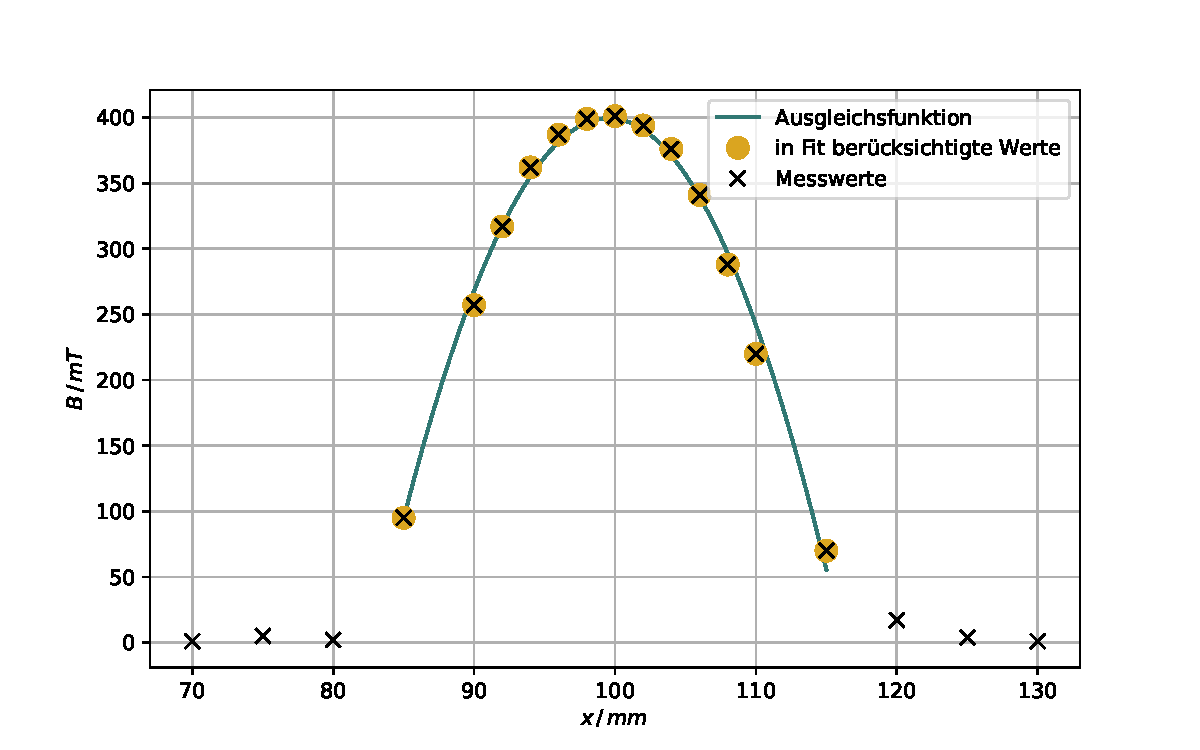
\includegraphics[width=0.9\textwidth]{figure/magnetfeld.pdf}
    \caption{Magnetfeldstärke $B$ in Abhängigkeit des Ortes $x$, wobei die $x$-Achse parallel zum Lichtstrahl verläuft und eine quadratische Ausgleichsfunktion.
    Die maximale Feldstärke entspricht der Feldstärke am Ort der Galliumarsenid-Probe.}
    \label{fig:magnetfeld}
\end{figure}
\FloatBarrier

% Bestimmung der effektiven Masse
\subsection{Effektive Masse der Leitungselektronen}
In diesem Abschnitt wird mittels gemessener Faraday-Rotation die effektive Masse der Leitungselektronen zweier n-dotierten Galliumarsenid-Proben bestimmt.
\autoref{tab:rein} beinhaltet die Messwerte der hochreinen Galliumarsenid-Probe und \autoref{tab:N1} der n-dotierten Galliumarsenid-Probe mit Ladungsträgerkonzentration $N_1 = \qty{1.2e18}{\centi\metre^2}$ bzw. \autoref{tab:N2} mit $N_2 = \qty{2.8e18}{\centi\metre^2}$.
Aus dem gemessenen Winkel $\theta_1$ bei angelegtem Magnetfeld $B_\text{max}$ und $\theta_2$ bei umgepolten Magnetfeld $-B_\text{max}$ ergibt sich der Rotationswinkel der Polarisationsebene nach
\begin{equation*}
    \theta = \frac{\theta_1 - \theta_2}{2} \, .
\end{equation*}
Die Rotationswinkel werden auf die Dicke $d$ der jeweiligen Probe normiert, dabei gilt für die Probendicke:
\begin{align}
    d_\text{rein} &= \qty{5.11}{\milli\metre} \\
    d_{N_1} &= \qty{1.36}{\milli\metre} \\
    d_{N_2} &= \qty{1.296}{\milli\metre}
\end{align}
Die berechneten Rotationswinkel $\theta$ bzw. normierten Rotationswinkel $\theta / d$ sind in den genannten Tabellen jeweils für die drei Proben zu finden.\\
%rein
\begin{table}
    \centering
    \caption{Gemessene Winkel $\theta_1, \theta_2$ für spezifische Wellenlängen $\lambda$ und der daraus resultierende Rotationswinkel $\theta$ bzw. $\theta/d$ für hochreines Galliumarsenid.}
    \label{tab:rein}
    \begin{tabular}{r r r r r}
        \toprule
        $\lambda \,/\, \unit{\micro\metre}$ & $\theta_1 \,/\, \unit{\degree}$ & $\theta_2 \,/\, \unit{\degree}$ & $\theta \,/\, \unit{rad}$ & $\frac{\theta}{d} \,/\, \frac{rad}{\unit{\metre}}$ \\
        \midrule
        1.060 & 89.08 & 65.50 & 0.206 & 40.275 \\
        1.290 & 81.03 & 66.67 & 0.125 & 24.535 \\
        1.450 & 78.43 & 68.33 & 0.088 & 17.248 \\
        1.720 & 78.88 & 68.33 & 0.092 & 18.017 \\
        1.960 & 72.92 & 65.50 & 0.065 & 12.666 \\
        2.156 & 69.17 & 64.50 & 0.041 & 7.970 \\
        2.340 & 49.48 & 44.23 & 0.046 & 8.966 \\
        2.510 & 33.58 & 29.97 & 0.032 & 6.176 \\
        2.650 & 65.10 & 60.75 & 0.038 & 7.429 \\
        \bottomrule
    \end{tabular}
\end{table}
%N_1
\begin{table}
    \centering
    \caption{Gemessene Winkel $\theta_1, \theta_2$ für spezifische Wellenlängen $\lambda$ und der daraus resultierende Rotationswinkel $\theta$ bzw. $\theta/d$ für n-dotiertes Galliumarsenid mit Ladungsträgerkonzentration $N_1 = \qty{1.2e18}{\centi\metre^2}$}
    \label{tab:N1}
    \begin{tabular}{r r r r r}
        \toprule
        $\lambda \,/\, \unit{\micro\metre}$ & $\theta_1 \,/\, \unit{\degree}$ & $\theta_2 \,/\, \unit{\degree}$ & $\theta \,/\, \unit{rad}$ & $\frac{\theta}{d} \,/\, \frac{rad}{\unit{\metre}}$ \\
        \midrule
        1.060 & 78.07 & 67.42 & 0.093 & 68.337 \\
        1.290 & 72.05 & 65.33 & 0.059 & 43.099 \\
        1.450 & 72.80 & 68.67 & 0.036 & 26.522 \\
        1.720 & 70.67 & 64.83 & 0.051 & 37.430 \\
        1.960 & 67.50 & 61.42 & 0.053 & 39.035 \\
        2.156 & 63.67 & 57.25 & 0.056 & 41.174 \\
        2.340 & 45.58 & 38.83 & 0.059 & 43.312 \\
        2.510 & 27.42 & 26.00 & 0.012 & 9.090 \\
        2.650 & 63.02 & 55.87 & 0.062 & 45.879 \\
        \bottomrule
    \end{tabular}
\end{table}
%N_2
\begin{table}
    \centering
    \caption{Gemessene Winkel $\theta_1, \theta_2$ für spezifische Wellenlängen $\lambda$ und der daraus resultierende Rotationswinkel $\theta$ bzw. $\theta/d$ für n-dotiertes Galliumarsenid mit Ladungsträgerkonzentration $N_2 = \qty{2.8e18}{\centi\metre^2}$}
    \label{tab:N2}
    \begin{tabular}{r r r r r}
        \toprule
        $\lambda \,/\, \unit{\micro\metre}$ & $\theta_1 \,/\, \unit{\degree}$ & $\theta_2 \,/\, \unit{\degree}$ & $\theta \,/\, \unit{rad}$ & $\frac{\theta}{d} \,/\, \frac{rad}{\unit{\metre}}$ \\
        \midrule
        1.060 & 78.83 & 65.33 & 0.118 & 90.903 \\
        1.290 & 72.83 & 61.25 & 0.101 & 77.997 \\
        1.450 & 75.50 & 68.50 & 0.061 & 47.135 \\
        1.720 & 76.17 & 66.08 & 0.088 & 67.896 \\
        1.960 & 69.92 & 61.25 & 0.076 & 58.357 \\
        2.156 & 69.17 & 60.50 & 0.076 & 58.357 \\
        2.340 & 52.00 & 39.83 & 0.106 & 81.925 \\
        2.510 & 27.22 & 12.58 & 0.128 & 98.534 \\
        2.650 & 67.98 & 54.50 & 0.118 & 90.790 \\      
        \bottomrule
    \end{tabular}
\end{table}
In \autoref{fig:theta_lam2} sind die normierten Rotationswinkel $\theta / d$ gegen das Quadrat der Wellenlänge $\lambda^2$ für die hochreine und beide n-dotierten Galliumarsenid-Proben aufgetragen.
\begin{figure}
    \centering
    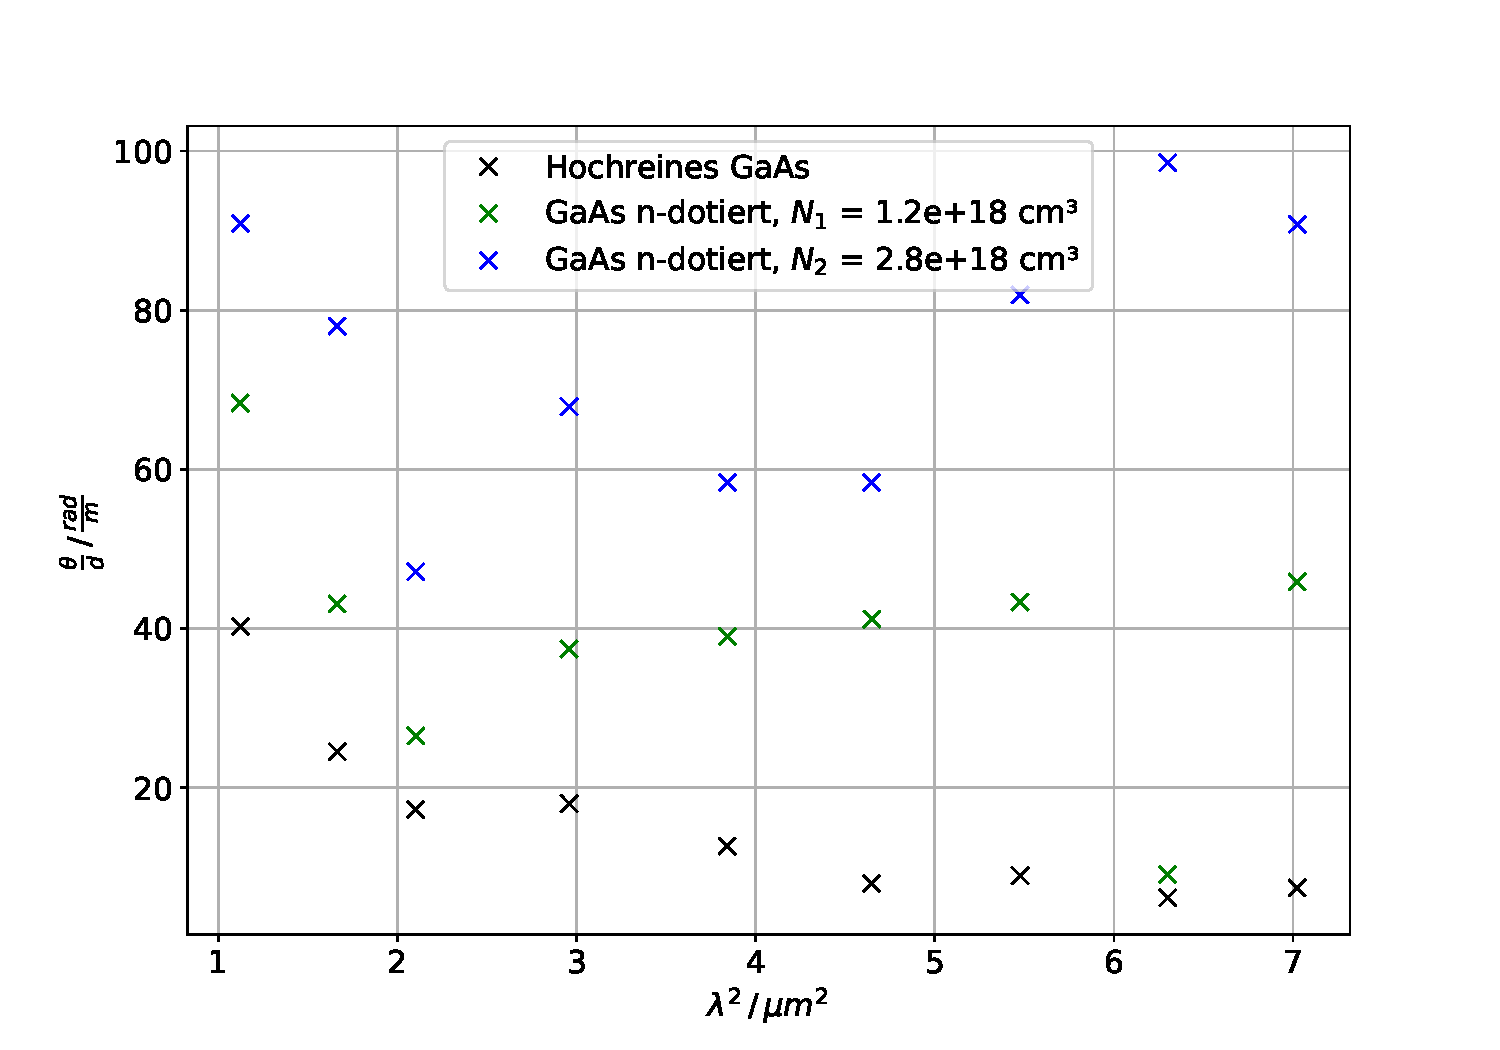
\includegraphics[width=0.8\textwidth]{figure/theta_lam2.pdf}
    \caption{Normierte Faraday-Rotation $\frac{\theta}{d}$ in Abhängigkeit der Wellenlänge zum Quadrat $\lambda^2$ für die hochreine und n-dotierten Galliumarsenid-Proben.}
    \label{fig:theta_lam2}
\end{figure}
Zur Bestimmung der effektiven Masse der Leitungselektronen darf nur die von diesen Elektronen verursachte Faraday-Rotation ausgewertet werden.
Dazu wird die Differenz von $\theta / d$ der n-dotierten Proben mit der hochreinen Probe gebildet.
Die resultierenden Winkel sind in Abhängigkeit von $\lambda^2$ in \autoref{fig:theta_dif_lam2} dargestellt.
\begin{figure}
    \centering
    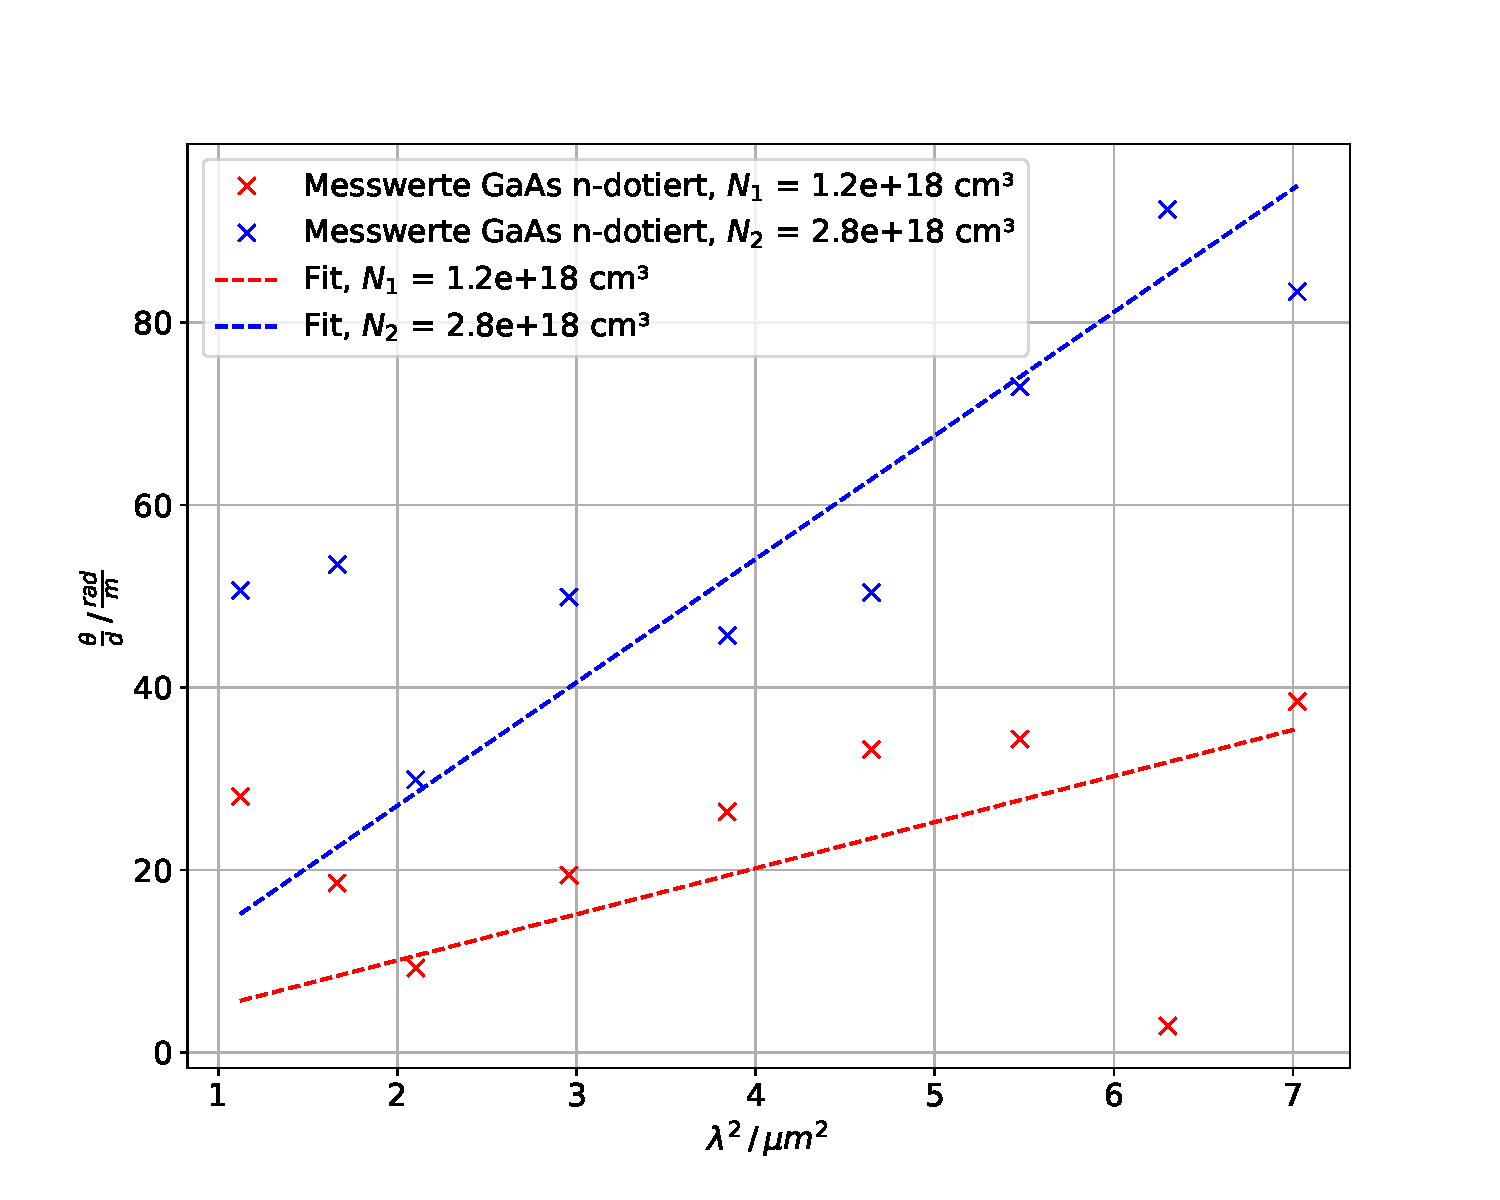
\includegraphics[width=0.8\textwidth]{figure/theta_lam2_dif.pdf}
    \caption{Differenz der normierten Faraday-Rotation der n-dotierten Proben mit der reinen Probe $\frac{\theta}{d}$ in Abhängigkeit der Wellenlänge zum Quadrat $\lambda^2$.
    Die Ausgleichsrechnung folgt der Funktion $\frac{\theta}{d} = a\cdot \lambda^2$.
    }
    \label{fig:theta_dif_lam2}
\end{figure}
Eine Ausgleichsrechnung der Form
\begin{equation}
    \frac{\theta}{d} = a \cdot \lambda^2
    \label{eqn:fit_lam2}
\end{equation}
wird mit den Wertepaaren $(\lambda^2, \theta / d)$ für die beiden n-dotierten Proben durchgeführt.
Der Parameter $a$ ergibt sich für die n-dotierte Probe mit Ladungsträgerkonzentration $N_1$ bzw. $N_2$ zu
\begin{align*}
    a_{N_1} &= \qty{5.1(11)e+12}{\frac{rad}{\metre^3}}, \\
    a_{N_2} &= \qty{1.35(14)e+13}{\frac{rad}{\metre^3}} \, . \\
\end{align*}
Die Ausgleichskurve ist für beide n-dotierten Proben in \autoref{fig:theta_dif_lam2} abgebildet.
Vergleicht man die Ausgleichsfunktion \autoref{eqn:fit_lam2} mit \autoref{eqn:THEORIE} und identifiziert den Fit-Parameter $a$, so folgt für die effektive Masse $m^*$%REF
\begin{align}
    a &= \frac{e_0^3}{8 \pi^2 \epsilon_0 c^3} \frac{1}{{m^*}^2} \frac{N B_\text{max}}{n} \\
    \Rightarrow m^* &= \sqrt{\frac{e_0^3}{8 \pi^2 \epsilon_0 c^3} \frac{1}{a} \frac{N B_\text{max}}{n}} \, .
\end{align}
Der Brechungsindex für Galliumarsenid $n = 3.346$ wird der Literatur \cite{GaAs_n} entnommen.
Die effektive Masse der Leitungselektronen wird somit auf
\begin{align*}
    m^*_{N_1} &= \qty{7.9(9)e-32}{\kilo\gram} &= \qty{0.086(9)}{m_e} \\
    m^*_{N_2} &= \qty{7.3(4)e-32}{\kilo\gram} &= \qty{0.081(4)}{m_e}
\end{align*}
bestimmt.
\FloatBarrier